\chapter{Descripción del Trabajo}
\label{cap:descripcionTrabajo}

En este capítulo abordaremos los aspectos tanto de diseño como de implementación de nuestra aplicación...TO BE CONTINUED

\section{Previos a la implementación}

\subsection{Reunión en el Centro de Tiflotecnología e Innovación de la ONCE}

\subsection{Exactitud de los beacons}

Antes de ponernos manos a la obra con la aplicación debíamos conocer cómo se comportaban los beacons en cuanto a distancias. La propia SDK de \textit{Kontakt} nos permite conocer qué beacons están en nuestro rango en un momento determinado y actualizar esa lectura cada cierto tiempo. Además tiene implementado un sistema de categorías en función de cómo de cerca o lejos esté el dispositivo. Las categorías son las siguientes:

\begin{itemize}
	\item IMMEDIATE: Si el dispositivo se encuentra a menos de 0,5m.
	\item NEAR: Si el dispositivo se encuentra entre los 0,5m y los 3m.
	\item FAR: Si el dispositivo se encuentra a más de 3m.
	\item UNKNOWN:The Unknown pone en la documentación...!!!!! ?
\end{itemize}

Para comprobar la fiabilidad y exactitud de estas medidas hicimos uso de pequeñas y simples aplicaciones que nos permitieron de manera rápida y visual ir comprobando las medidas leídas con las reales tanto dentro de la facultad como dentro de otros edificios (nuestras propias casas).

\subsubsection{Aplicación miniapp}
Esta aplicación fue la primera toma de contacto con los beacons, queríamos una aplicación sencilla y visual que nos indicara la categoría de proximidad de los beacons. Como podemos ver en la Figura \ref{fig:miniapp}, los beacons considerados se encuentran debajo del panel de categorías y la categoría se resalta en verde. La lectura que se hace de los beacons se va actualizando cada $x$ tiempo establecido. 

La idea de esta aplicación fue la de establecer el grado de confianza que podíamos tener en las categorías ofrecidas por la SDK de \textit{Kontakt}. El resultado fue muy positivo puesto que, a pesar de que las distancias fluctuaban, la categoría se asignaba correctamente sin grandes fluctuaciones. 

\begin{figure}[t]
	\centering
	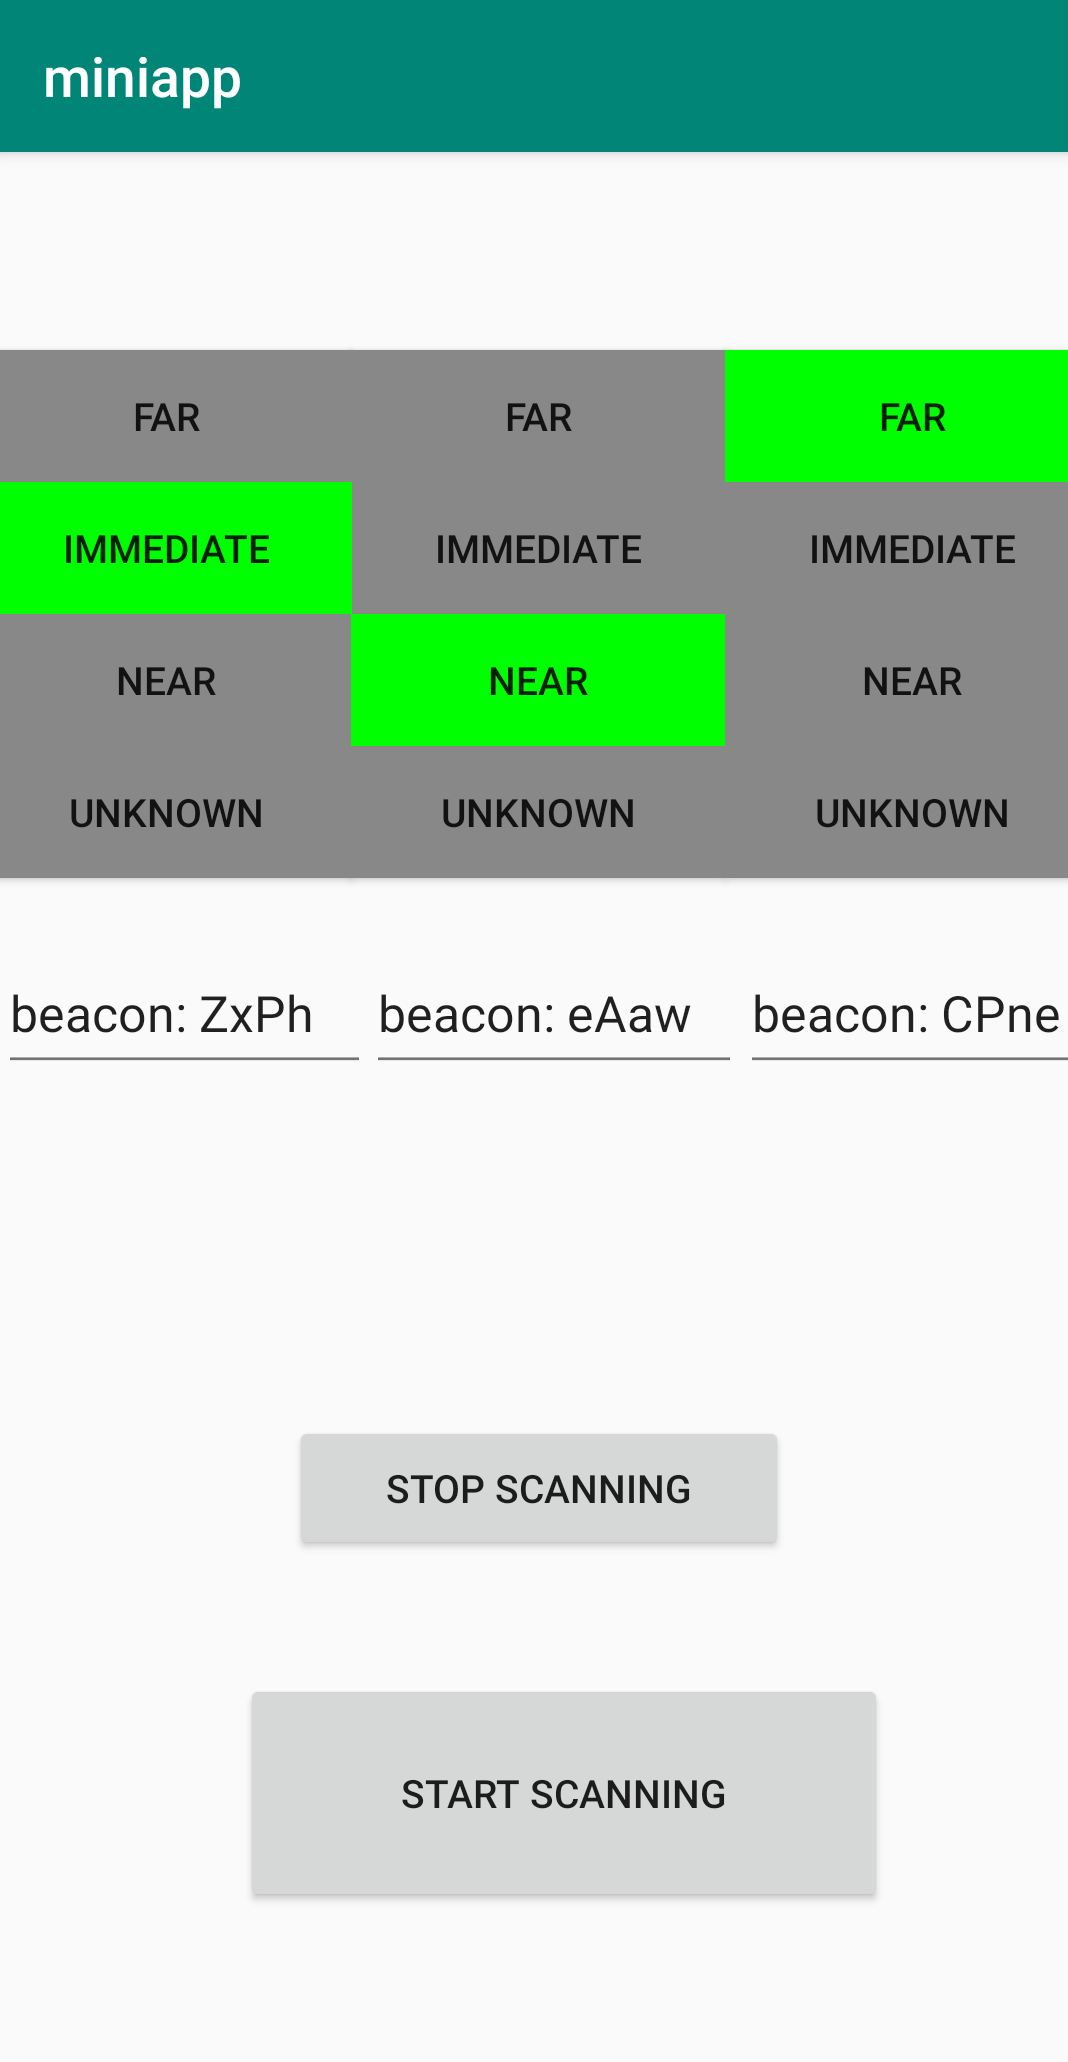
\includegraphics[width=0.4\textwidth]{Imagenes/Descripciondeltrabajo/miniapp}
	\caption{Interfaz de la aplicación miniapp. }
	\label{fig:miniapp}
\end{figure}

\subsubsection{Aplicación cuadrantes v1}
En la Figura \ref{fig:cuadrantesv1} vemos la interfaz principal de la aplicación \textit{cuadrantes v1}, esta fue diseñada, en inicio, para saber a qué distancia debían estar los beacons y poder así dividir las distintas plantas de la facultad en cuadrantes, de esta manera podríamos construir un grafo cuyos nodos fueran estos cuadrantes y, que representara el mapa de la facultad.

Es una aplicación muy sencilla, cuya función es recoger cada cierto tiempo, en la figura lo hace cada dos segundos, la señal de los beacons que están a su alcance, mostrar la categoría de su distancia y la distancia a la que se encuentran en metros. La razón por la que llevamos un registro de qué está en el rango cada cierto tiempo es que notamos que las distancias fluctuaban, notoriamente en algunos casos, y quisimos hacer un estudio previo al desarrollo de la aplicación.

\begin{figure}[t]
	\centering
	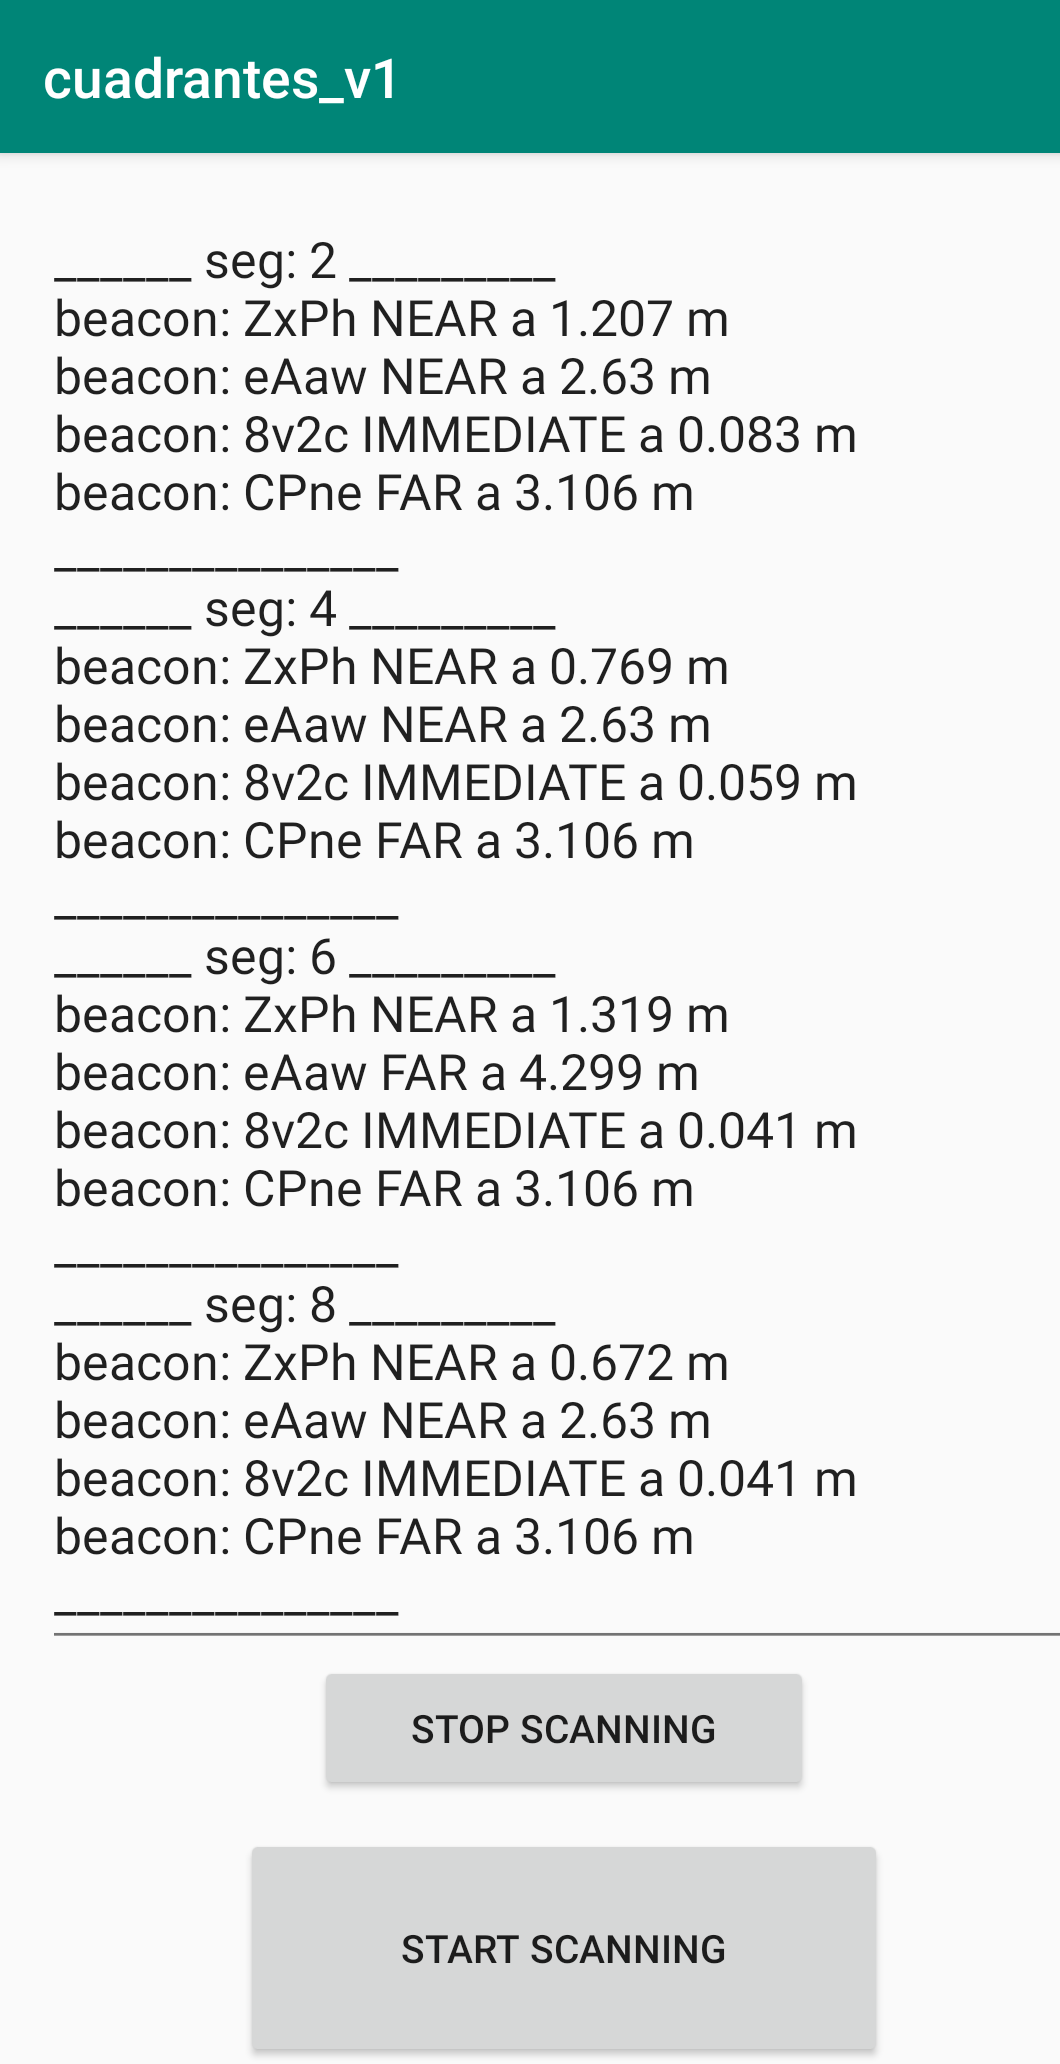
\includegraphics[width=0.4\textwidth]{Imagenes/Descripciondeltrabajo/cuadrantes_v1}
	\caption{Interfaz de la aplicación cuadrantes v1.}
	\label{fig:cuadrantesv1}
\end{figure}


\subsubsection{Resultados}

A continuación presentamos los resultados de las distintas mediciones realizadas. Veamos primero los gráficos, en los que podemos ver cómo se comportan los beacons si comparamos la medida real con la dada por la aplicación. 

En la Figura \ref{fig:dist_CPne} vemos las lecturas que nos ha dado la aplicación \textit{cuadrantes v1} cuando hemos leído las distancias del beacon con identificador CPne. De esta gráfica destacamos que a grandes distancias, en este caso 5m, la distancia comienza a no ser muy fiable, a la par que muy fluctuante. Sin embargo, podemos ver cómo la medida a dos metros de distancia es la bastante exacta, fluctúa en menos de un metro a lo largo de casi toda la medición. Por último, la medición a menos de un metro, que se corresponde con la línea amarilla presenta fluctuaciones muy pequeñas, poco relevantes para nuestra aplicación. 

\begin{figure}[t]
	\centering
	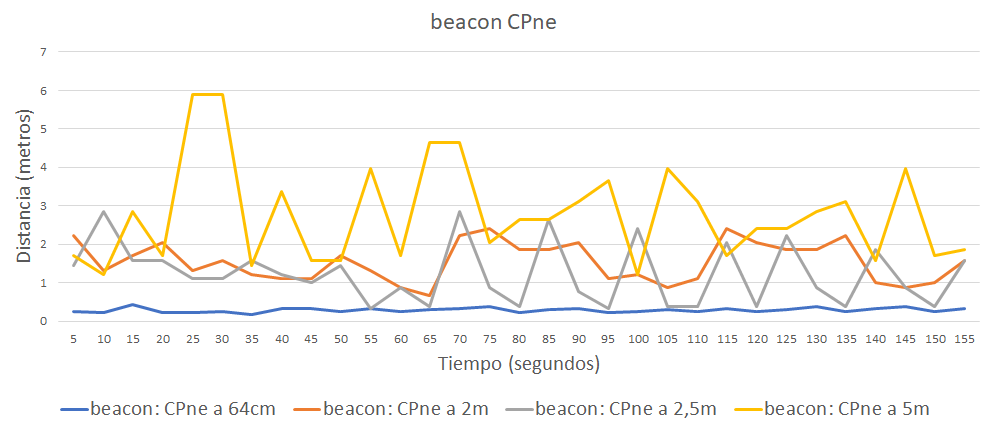
\includegraphics[width=0.7\textwidth]{Imagenes/Descripciondeltrabajo/dist_CPne}
	\caption{Gráfico con las distancias medidas al beacon CPne. }
	\label{fig:dist_CPne}
\end{figure}

En el caso de la Figura \ref{fig:dist_eAaw} el comportamiento es similiar, a pesar de que tenemos un par de picos importantes en los primeros segundos de medición. La Figura \ref{fig:dist_8v2c} recoge tres mediciones distintas para una misma distancia, cada una de ellas recoge unos valores distintos y bastante bajos, lejos de los aproximadamente 4 metros reales. Una posible explicación a este fenómeno nos lo puede dar la Figura \ref{fig:dist_conjunto}, que recoge la medición de dos beacons situados a la misma distancia y uno encima del otro. Como vemos, la medición del beacon situado abajo es bastante más baja, en comparación. Esto nos advierte de que la señal bluetooth es bastante dependiente de los obstáculos, el entorno, ¡hasta las condiciones meteorológicas!. 


\begin{figure}[t]
	\centering
	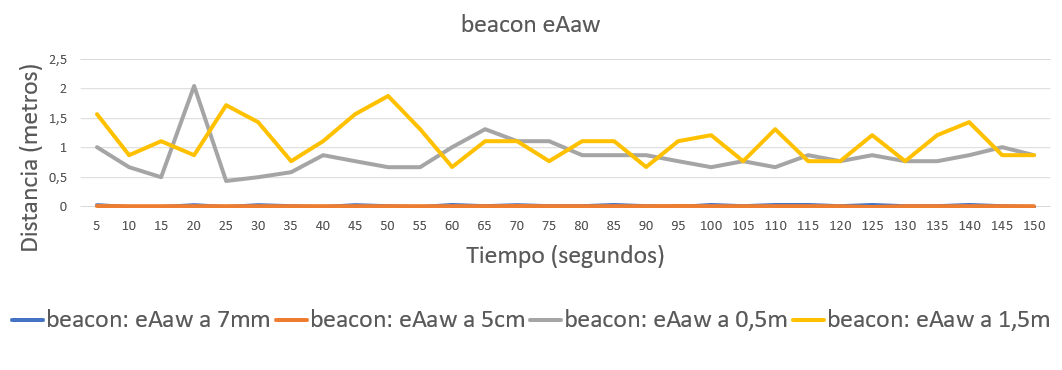
\includegraphics[width=0.7\textwidth]{Imagenes/Descripciondeltrabajo/dist_eAaw}
	\caption{Gráfico con las distancias medidas al beacon eAaw. }
	\label{fig:dist_eAaw}
\end{figure}


\begin{figure}[t]
	\centering
	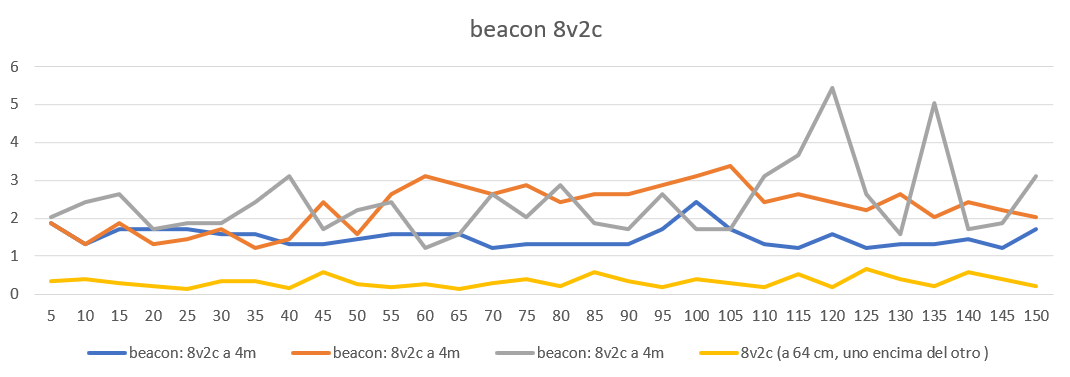
\includegraphics[width=0.7\textwidth]{Imagenes/Descripciondeltrabajo/dist_8v2c}
	\caption{Gráfico con las distancias medidas al beacon 8v2c. }
	\label{fig:dist_8v2c}
\end{figure}

\begin{figure}[t]
	\centering
	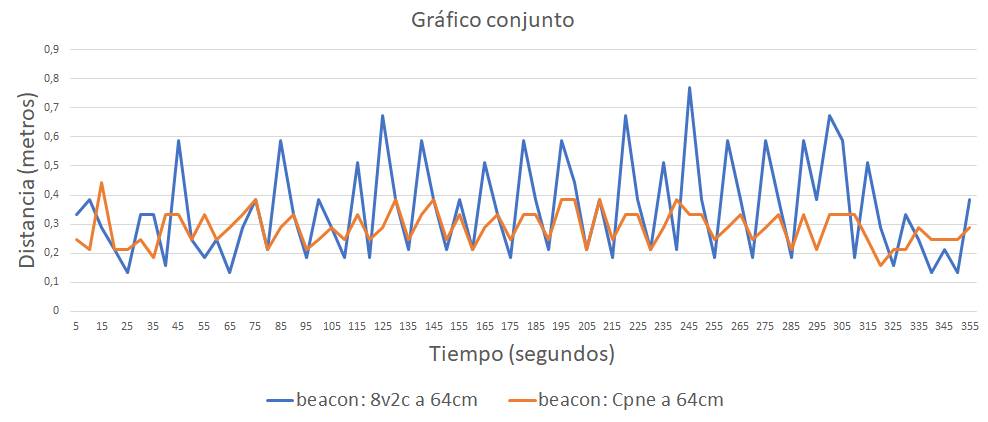
\includegraphics[width=0.7\textwidth]{Imagenes/Descripciondeltrabajo/dist_conjunto}
	\caption{Gráfico con las distancias medidas conjuntas de los beacons 8v2c y CPne, estando uno sobre otro. }
	\label{fig:dist_conjunto}
\end{figure}


\subsubsection{Mediciones en lugares clave de la facultad}

También se realizaron mediciones sobre posibles posiciones reales de los beacons dentro de la facultad. Para ello se colocaron estos beacons en lugares clave, como las puertas de la calle, de las aulas, delegación de alumnos, o secretaría, y, con ayuda de nuestra app \textit{cuadrantes v1} se recogieron los datos medidos, que se muestran a continuación: 

LOS DATOS QUE VIENEN ESTÁN EN EL ARCHIVO medicionesFacltad.txt QUIERO PREGUNTAR CÓMO METER ESTO Y SI METERLO TODO, en cualquier caso creo que habría que poner el mapa y donde están los beacons y todo eso.
